\section{Segmentation du texte}
La phase de segmentation est la première phase du processus et l'extraction des données.
L'algorithme est développé sur les vingt premières pages du registre. Lorsque celui-ci atteint une précision suffisante sur cet ensemble de données réduit, il est alors testé et évalué sur l'ensemble du registre ; au besoin, il est corrigé ou amélioré.

Lorsque le document source est importé dans l'environnement de développement en format texte (\textit{.txt}), ce dernier va découper le contenu textuel en petites chaînes de caractères au niveau des espaces et stocker celles-ci dans un vecteur de type caractère. Ceci présente l'avantage que chaque mot ou marqueur de structure peut être désigné par sa position à l'intérieur du vecteur. Par conséquent, capturer une section spécifique du texte nécessite uniquement de pouvoir déterminer les positions du début et de fin de celle-ci au sein du vecteur.  

Le document source est donc transformé en un vecteur \textit{T} de 15390 éléments.
Quant aux procédés de détection et de capture des différentes parties du document source, ils peuvent être formalisés par les expressions régulières et les formules du tableau \ref{regexSeg}.
\vspace{0,5cm}
\renewcommand{\arraystretch} {1.5}
\begin{table}[ht]
    \centering
    \begin{tabular}{|l|c|l|}
        \hline \textbf{Objet} & \textbf{Symbole} & \textbf{Regex ou Formule}  \\
        \hline \hline Marqueur d'escroete & $mEs$ & \textasciicircum[IV]+([1-9])?\$ \\
        \hline Section d'escroete & $sEs$& $ sEs_{[n]} =  T[mEs_{[n]}:mEs_{[n+1]}-1] $\\
        \hline  Définition d'escroete & $dEs $& $ dEs_{[n]} = T[mEs_{[n]}:mCo_{[1]}-1] $\\
        \hline  Marqueur de connétablie & $mCo$ & [0-9]+° \\
        \hline Section de connétablie & $sCo $& $sCo_{[n]} =  sEs[mCo_{[n]}:mCo_{[n+1]}-1] $\\
        \hline Définition de connétablie & $dCo$ & $ dCo_{[n]} = sEs[mCo_{[n]}:mRdV_{1]}-1] $\\
            & & $ dCo_{[n]} = sEs[mCo_{[n]}:mRe_{1]}-1] $ \\
        \hline  Marqueur de rang de voie & $mRdv$ & \textasciicircum[AB]\$ \\
        \hline Section de rang de voie & $sRdv$ &$ sRdv_{[n]} = sCo[mRdv_{[n]}:mRdv_{[n+1]}-1] $\\
        \hline Marqueur de rente & $mRe$ & [0-9]\{2,\}. \\
        \hline Section de rente & $sRe$& $sRe_{[n]} = sRdv[mRe_{[n]}:mRe_{[n+1]}-1]$ \\
            & &  $ sRe_{[n]} = sCo[mRe_{[n]}:mRe_{[n+1]}-1]$ \\
        \hline
    \end{tabular}
    \caption{Formules et expression régulières pour la segmentation du registre}
    \label{regexSeg}
\end{table}
\vspace{0,5cm}
\subsection{Correction des numéros de rente}
Une fois les numéros de rentes extraits, ils doivent encore être corrigés pour défaire le numéro de rente du numéro de rente successif au sein d'une même connétablie. Cette correction est particulièrement importante, car en plus de rétablir l'information topographique contenue dans le numéro de rente, elle permet d'éviter le risque d'avoir des doublons créés par la concaténation des deux numéros lors de la conversion du document source en format texte(\textit{.txt}).
Pour cela, un compteur est initialisé  dans une variable globale à chaque nouvelle connétablie traitée (lorsque la fonction \textit{connetablieExtract()} est appelée). 
Cette variable globale est utilisée en argument de la fonction \textit{str\_replace()} afin d'insérer un caractère <<.>> entre les deux numéros. La variable globale est ensuite incrémentée.

La difficulté arrive avec les irrégularités dans l'ordre des connétablies :si de manière générale les connétablies sont classées en fonction de leur numéro, par ordre croissant, certaines  sont divisées en plusieurs parties dans le registre avec une mention <<bis>>  attachée  à leur numéro.  Ces connétablies sont considérées à part entière dans le tableau de donnée, car elles peuvent correspondre à une particularité topographique qui les distingue du reste de la connétablie. Cependant, le <<numéro de rente successif au sein d'une même connétablie>> doit se continuer à travers les différentes parties de la connétablie,  et non, se réinitialiser. Pour remédier à cela, 
la fonction \textit{str\_detect()} est utilisée  afin de vérifier si le numéro de la connétablie actuellement traité contient une particule \textit{bis}. Auquel cas, la fonction \textit{str\_extract()} est employée avec l'expression régulière \textit{<<\textbackslash d+°>>} et la fonction \textit{nrow()} pour de compter le nombre de rentes liées à ce numéro de connétablie et incrémenter la variable globale de comptage en  fonction. Ce processus est illustré par la figure \ref{schemaNumRenteCorr}.
\begin{figure}
    \centering
    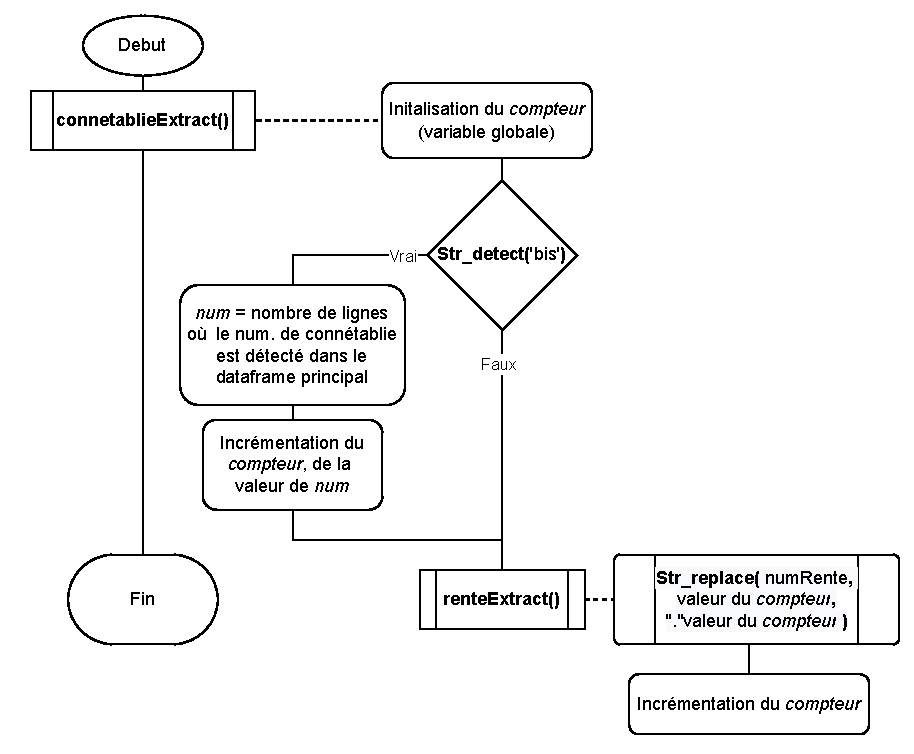
\includegraphics{3.Results/Img/numRente_corr.drawio.pdf}
    \caption{Organigramme de la correction des numéros de rentes}
    \label{schemaNumRenteCorr}
\end{figure}


\subsection{Évaluation}
Le script de segmentation nous retourne toutes les informations extraites depuis le document source dans un tableau de données consultable dans la partie \textit{Annexes} du mémoire. 
\begin{table}[ht]
    \centering
    \begin{tabular}{|l||c|c|c|c|c|}
        \hline		&	\textbf{Correct}	&	\textbf{Incorrect}	&	\textbf{NA}	&	\textbf{Typo}	&	\textbf{Total} \\
        \hline
        \hline	Numéros des escroetes	&	13	&	0	&	0	&	0	&	13\\
        \hline	Définitions des escroetes	&	5	&	0	&	2	&	5	&	12 \\
        \hline	Numéros des connétablies	&	85	&	0	&	0	&	0	&	85 \\
        \hline	Définition des connétablies	&	83	&	0	&	0	&	1	&	84 \\
        \hline	Numéro des rentes	&	308	&	0	&	0	&	8	&	316 \\
        \hline	Section des rentes	&	313	&	0	&	0	&	3	&	316 \\
        \hline
    \end{tabular}
    \caption{Résultats de la segmentation du document source.}
    \label{eval_seg}
\end{table}

Les résultats de cette phase de segmentation sont relativement satisfaisants, la très grande majorité des informations sont extraites avec succès comme le montre le tableau \ref{eval_seg}. 
Quelques informations sont manquantes par rapport à la définition des escroetes III et IV. Ces lacunes sont dues à une irrégularité dans le registre. Ces 2 erreurs affectent au total 67 lignes dans le tableau de données principal, cependant, ce n'est pas trop grave étant donné que les numéros d'escroetes sont présents et qu'ils suffisent à identifier la zone topographique des rentes. En dehors de cela, quelques erreurs de typographies sont remarquées, principalement dans les définitions des escroetes et dans les sections des rentes. Ces erreurs concernent les dernières pages du registre de rentes qui présentent moins de régularité que le reste du document.






